\documentclass[11pt, letterpaper]{article}
\usepackage[utf8]{inputenc}
\usepackage[letterpaper, margin=0.5in]{geometry}
\usepackage{amsmath}
\usepackage{amssymb}
\usepackage{amsthm}
\usepackage{wrapfig}
\usepackage{graphicx}
\usepackage[font=scriptsize]{caption}
\usepackage{subcaption}
\graphicspath{ {./statics/} }
\captionsetup{justification=raggedright, singlelinecheck=false}


\title{STA 602 HW2}
\author{Ryan Tang}
\date{September 11th 2022}

\begin{document}
\maketitle

\section{Excerise 3.1}
\paragraph{(a)}
\begin{align*}
    Y_{i\in N} \overset{iid}{\thicksim} Bernoulli(\theta) && N &= 100 \\
    p(y_1, y_2 \dots y_{100}) &= \prod_{i=1}^{100} \mathbb{I}(y_i=1)\theta + \mathbb{I}(y_i=0)(1-\theta) \\
        &= {\theta^{N_1}(1-\theta)}^{N_0} && N_1 = \sum_{i=1}^{100} \mathbb{I}(y_i=1) \\
    p(\sum_i^{100} y_i | \theta) &= {100 \choose N_1} {\theta^{N_1}(1-\theta)}^{N_0}
\end{align*}

\paragraph{(b) $\thicksim$ (e)}

\begin{figure*}[!b]
    \centering
    \begin{subfigure}{.49\textwidth}
        \centering
        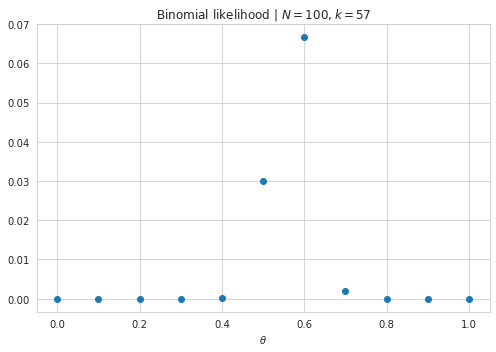
\includegraphics[scale=0.44]{hw2_binom1.png}
        \caption{plot for 3.1.b --- Likelihood Distribution $p(\mathbf{x}=57|\theta, n=100)$}
    \end{subfigure} %    
    \begin{subfigure}{.49\textwidth}
        \centering
        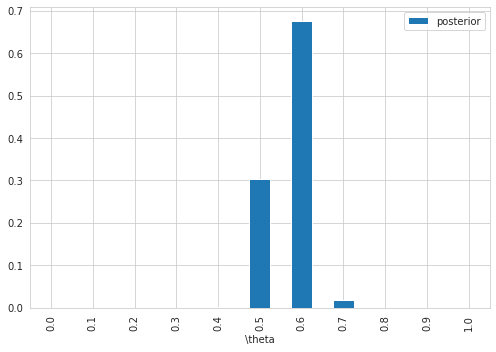
\includegraphics[scale=0.44]{hw2_binom_post1.png}
        \caption{plot for 3.1.c --- Posterior Distribution $p(\theta|\mathbf{x})$}
    \end{subfigure}
    \begin{subfigure}{.49\textwidth}
        \centering
        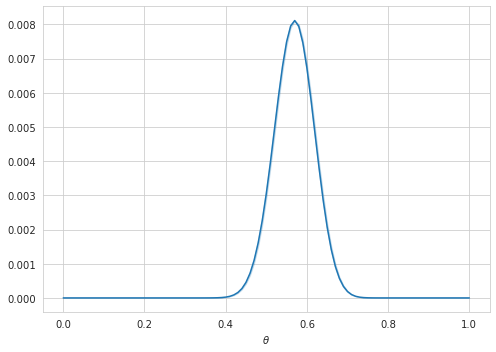
\includegraphics[scale=0.44]{hw2_3.1.d.png}
        \caption{plot for 3.1.d --- Posterior Distribution $p(\theta|\mathbf{x})$ on continuous Uniform prior}
    \end{subfigure}
    \begin{subfigure}{.49\textwidth}
        \centering
        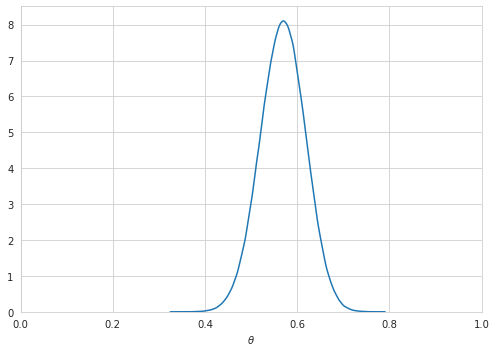
\includegraphics[scale=0.44]{hw2_3.1.e.png}
        \caption{plot for 3.1.d --- $Beta(58, 44)$ Density}
    \end{subfigure}
\end{figure*}

To summarize below, all 4 plots, (a) and (b), are just the coalesced version for Bayesian belief updates. (c) shows the posterior
after applying to the Uniform prior. Lastly, (e) confirms that the Beta distribution is conjugate to the Binomial likelihood, and
the Uniform prior, equivalent to a $Beta (1, 1)$ distribution, has been treated as a weak prior belief with only 2 sample sizes.
Hence, the resulting posterior is also a Beta distribution.

\section{Excerise 3.2}

\begin{wrapfigure}{l}{0.5\textwidth}
    \begin{center}
        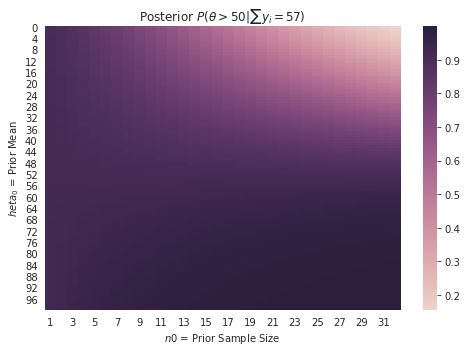
\includegraphics[scale=0.56]{hw2_3.2.png}
    \end{center}
\end{wrapfigure}

To the left is the sensitivity analysis on how various prior beliefs would affect the resulting posterior belief after
observing the survey data, $N=100, \sum y_i = 57$.
\begin{itemize}
    \item If one has a strong prior belief, top right corner, it is hard to move the prior without significant evidence.
    \item On the contrary, suppose one does not hold a strong belief, bottom left corner, he or she should take the survey evidence strongly.
\end{itemize}


\section{Excerise 3.4}


\end{document}